\documentclass[12pt]{article}

\usepackage[margin=0.7in]{geometry}
\usepackage{amsfonts, amssymb, amsmath}
\usepackage[none]{hyphenat}
\usepackage{fancyhdr}
\usepackage{float}
\usepackage{setspace}
\usepackage{graphicx}
\usepackage{hyperref}
\usepackage[table]{xcolor}
\usepackage{multirow}
\usepackage{color}
\usepackage{listings}

\pagestyle{fancy}
\fancyhead{}
\fancyfoot{}
\fancyhead[L]{\MakeUppercase{CH1202 Expt. No.: 01}}
\fancyhead[R]{\slshape Priyanshu Mahato: \href{mailto:pm21ms002@iiserkol.ac.in}{\color{purple}pm21ms002@iiserkol.ac.in}}
\fancyfoot[C]{\thepage}

\renewcommand{\footrulewidth}{1pt}
% \renewcommand{\baselinestretch}{1.2}
\renewcommand\thesection{\arabic{section}}

\setlength{\headheight}{16pt}
\setlength{\parindent}{0em}
\setlength{\parskip}{1.5em}

\lstset{frame=tb,
	language=Python,
	aboveskip=3mm,
	belowskip=3mm,
	showstringspaces=false,
	columns=flexible,
	basicstyle={\small\ttfamily},
	numbers=none,
	numberstyle=\tiny\color{gray},
	keywordstyle=\color{blue},
	commentstyle=\color{dkgreen},
	stringstyle=\color{mauve},
	breaklines=true,
	breakatwhitespace=true,
	tabsize=3
}

\definecolor{dkgreen}{rgb}{0,0.6,0}
\definecolor{gray}{rgb}{0.5,0.5,0.5}
\definecolor{mauve}{rgb}{0.58,0,0.82}
\definecolor{ChadDarkBlue}{rgb}{.1,0,.2}  
\definecolor{ChadBlue}{rgb}{.1,.1,.5}  
\definecolor{ChadRoyal}{rgb}{.2,.2,.8}  
%\definecolor{ChadGreen}{rgb}{0,.35,.1}
%\definecolor{ChadGreen}{rgb}{0,.5,.25}  % Too bright
%\definecolor{ChadGreen}{rgb}{0,.4,.2}    % Still too bright
\definecolor{ChadGreen}{rgb}{0.5, 0, 0.2}    % Dark Green
%\definecolor{ChadRed}{rgb}{.8,.1,.2}    % Too bright
\definecolor{ChadRed}{rgb}{.5,0,.5}  % purple

\begin{document}
	\thispagestyle{empty}
	\begin{titlepage}
		\begin{center}
			\vspace{2cm}
			\huge\textbf{CH1202}\\
			\vspace{1cm}
			\large\textbf{Chemistry Laboratory II}
			\vfill
			\line(1, 0){470}\\[14pt]
			\huge\textbf{\color{ChadBlue}\sffamily Experiment Number - 01}\\[10pt]
			\Large\textbf{\color{mauve}\sffamily Determination of the Isoelectric Point of an Amino Acid}\\[14pt]
			\line(1, 0){470}
			\vfill
			By: Priyanshu Mahato (\href{mailto:pm21ms002@iiserkol.ac.in}{\emph{\color{dkgreen}pm21ms002@iiserkol.ac.in}})\\
			Roll No.: pm21ms002\\
			\today
		\end{center}
	\end{titlepage}

	\section{Aim}
	
	To determine the isoelectric point of an amino acid.
	
	\section{Apparatus Required}
	
	\begin{enumerate}
		\item pH meter
		\item Beaker
		\item Burette
		\item Pipette
		\item Glass Rod
		\item Spatula
	\end{enumerate}

	\section{Reagents and Materials}
	
	\begin{enumerate}
		\item Potassium Hydrogen Phthalate
		\item Glycine
		\item Alanine
		\item Hydrochloric Acid
		\item Sodium Hydroxide
		\item Phenolphthalein
	\end{enumerate}

	\section{Equations}
	
	\emph{Henderson-Hasselbach Equation:-}
	
	$$pK_{a} = pH + \log\frac{[HA]}{[A^{-1}]}$$
	
	\begin{figure}[H]
		\centering
		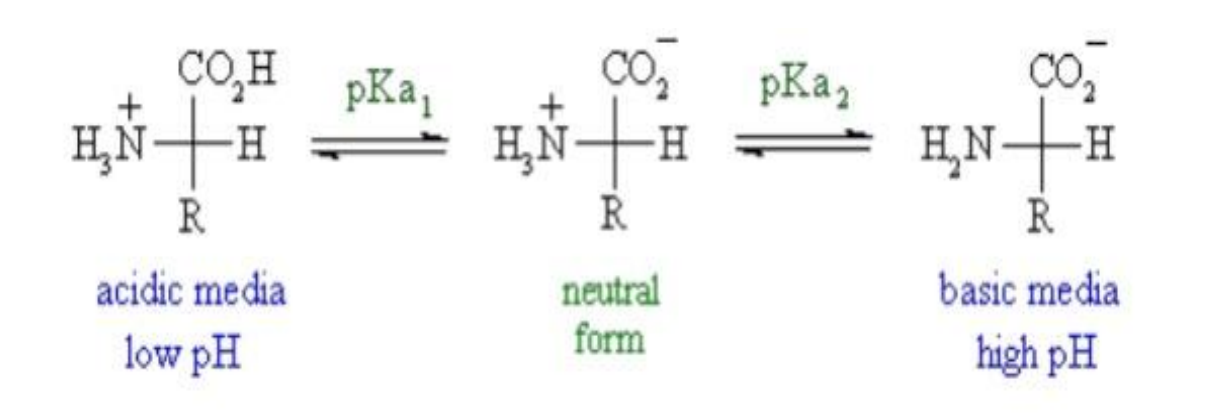
\includegraphics[scale=0.6]{picture}
	\end{figure}

	\emph{To find $pI$ (Isoelectric Point):-}
	
	$$pI = \frac{pK_{a_{1}} + pK_{a_{2}}}{2}$$
	
	$$Moles\ of\ Acid = V_{Base}\ (at\ Equivalence\ Point) \times M_{Base}$$
	
	\section{Datasets}
	
	Room Temperature $= 25^{\circ}C$
	
	\begin{table}[H]
		\centering
		\begin{tabular}{|l|l|l|}
			\hline
			Weight Taken (g) & Weight to be taken (g) & Strength of KHP solution \\ \hline
			2.050            & 2.04222                & 20.5 $gL^{-1}$             \\ \hline
		\end{tabular}
	\caption{ Preparation of 100 
		mL standard 0.1 N KHP 
		solution.}
	\end{table}

	Molecular weight of KHP $= 204.222 gmol^{-1}$\\
	Strength = $\dfrac{(mass\ of\ solute\ in\ g)}{Litre\ (L)}$ = $\dfrac{2.05 g}{0.1 L}$ = 20.5 $gL^{-1}$
	
\begin{table}[H]
	\centering
	\begin{tabular}{|l|l|lll|l|l|}
		\hline
		\multirow{2}{*}{Sl. No.} &
		\multirow{2}{*}{Volume of KHP (mL)} &
		\multicolumn{3}{l|}{Burette Reading (mL)} &
		\multirow{2}{*}{\begin{tabular}[c]{@{}l@{}}Average \\ Volume (mL)\end{tabular}} &
		\multirow{2}{*}{\begin{tabular}[c]{@{}l@{}}Strength of \\ NaOH Solution\end{tabular}} \\ \cline{3-5}
		&    & \multicolumn{1}{l|}{Initial} & \multicolumn{1}{l|}{Final} & Difference &                         &                                  \\ \hline
		1 & 10 & \multicolumn{1}{l|}{0}       & \multicolumn{1}{l|}{10.1}  & 10.1       & \multirow{3}{*}{10.167} & \multirow{3}{*}{3.949 $gL^{-1}$} \\ \cline{1-5}
		2 & 10 & \multicolumn{1}{l|}{0}       & \multicolumn{1}{l|}{10.2}  & 10.2       &                         &                                  \\ \cline{1-5}
		3 & 10 & \multicolumn{1}{l|}{0}       & \multicolumn{1}{l|}{10.2}  & 10.2       &                         &                                  \\ \hline
	\end{tabular}
	\caption{Standardization of 
	NaOH solution using 
	standard KHP solution}
\end{table}

	Molecular weight of NaOH = 39.997 $gmol^{-1}$
	
	$$\frac{S_{1}\cdot V_{1}}{M_{1}} = \frac{S_{2}\cdot V_{2}}{M_{2}}$$
	
	S1 = 20.5 $gL^{-1}$\\
	V1 = 10 mL = 0.01 L \\
	V2 = 10.167 mL = 0.010167 L\\
	
	so, $\dfrac{20.5 \times 0.01}{204.222} = \dfrac{S_{2}
	\times 0.010167}{39.997} \Rightarrow S2= 3.949 gL^{-1}$

	Volume of 
	amino acid = 25 mL
	
	\begin{figure}[H]
		\centering
		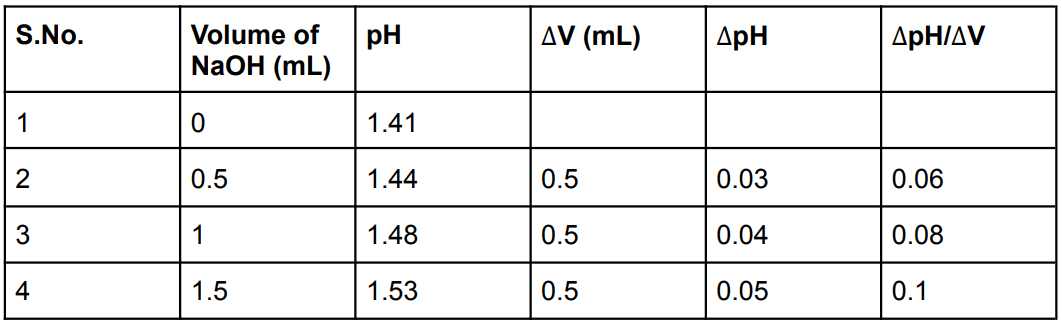
\includegraphics[scale=0.7]{table1}
	\end{figure}
	\begin{figure}[H]
		\centering
		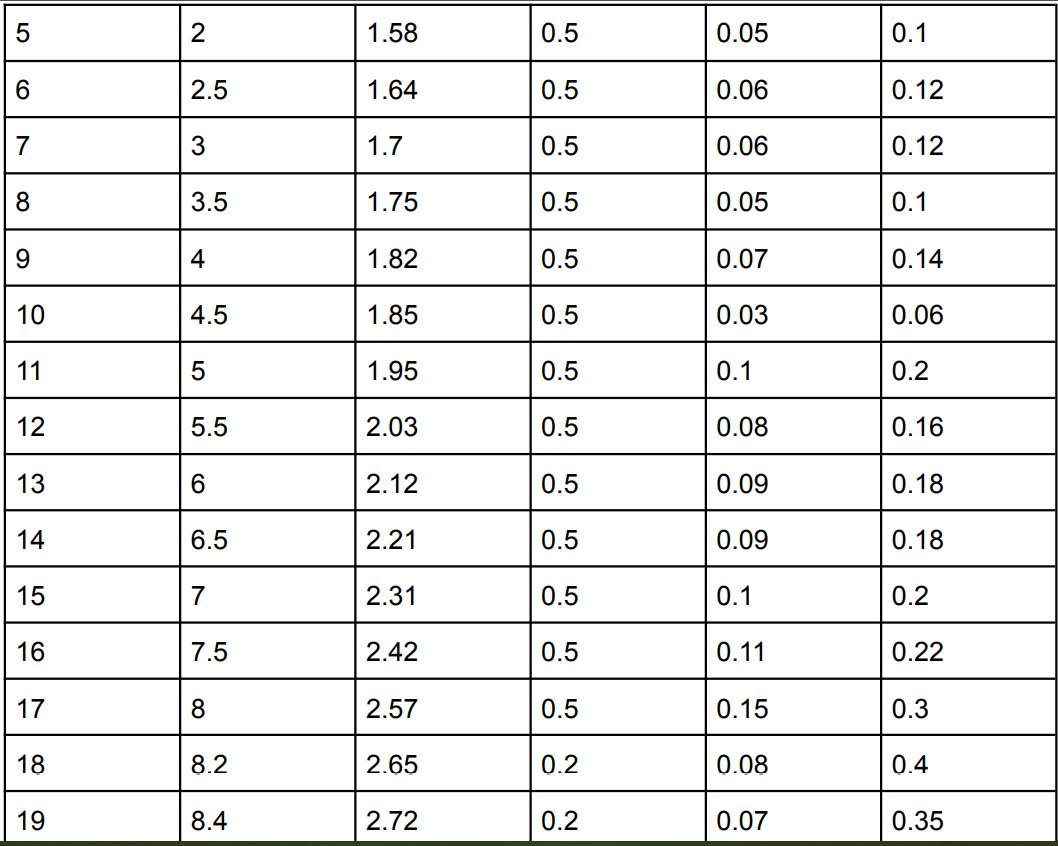
\includegraphics[scale=0.7]{table2}
	\end{figure}
	\begin{figure}[H]
		\centering
		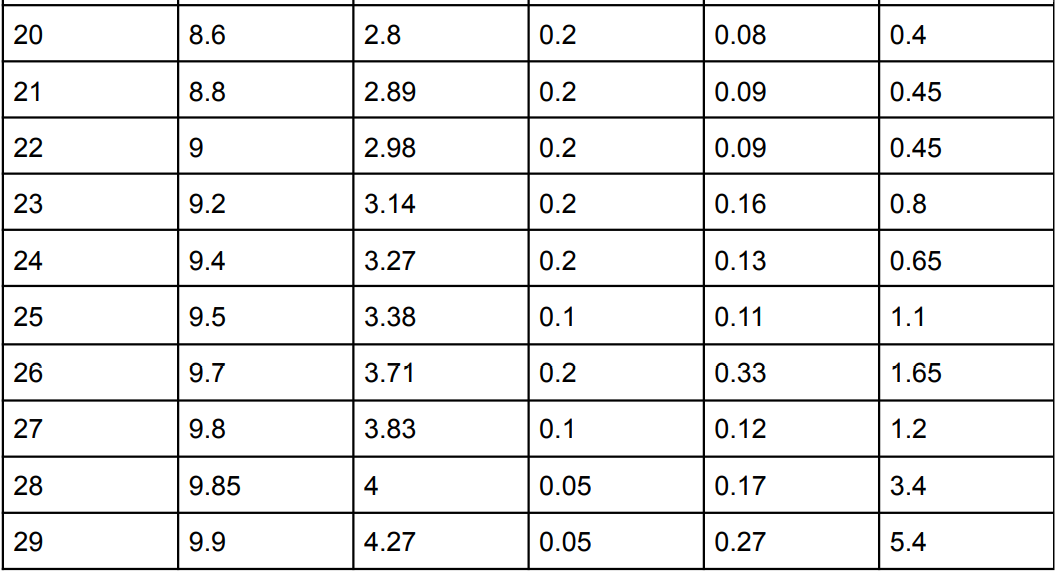
\includegraphics[scale=0.7]{table3}
	\end{figure}
	\begin{figure}[H]
		\centering
		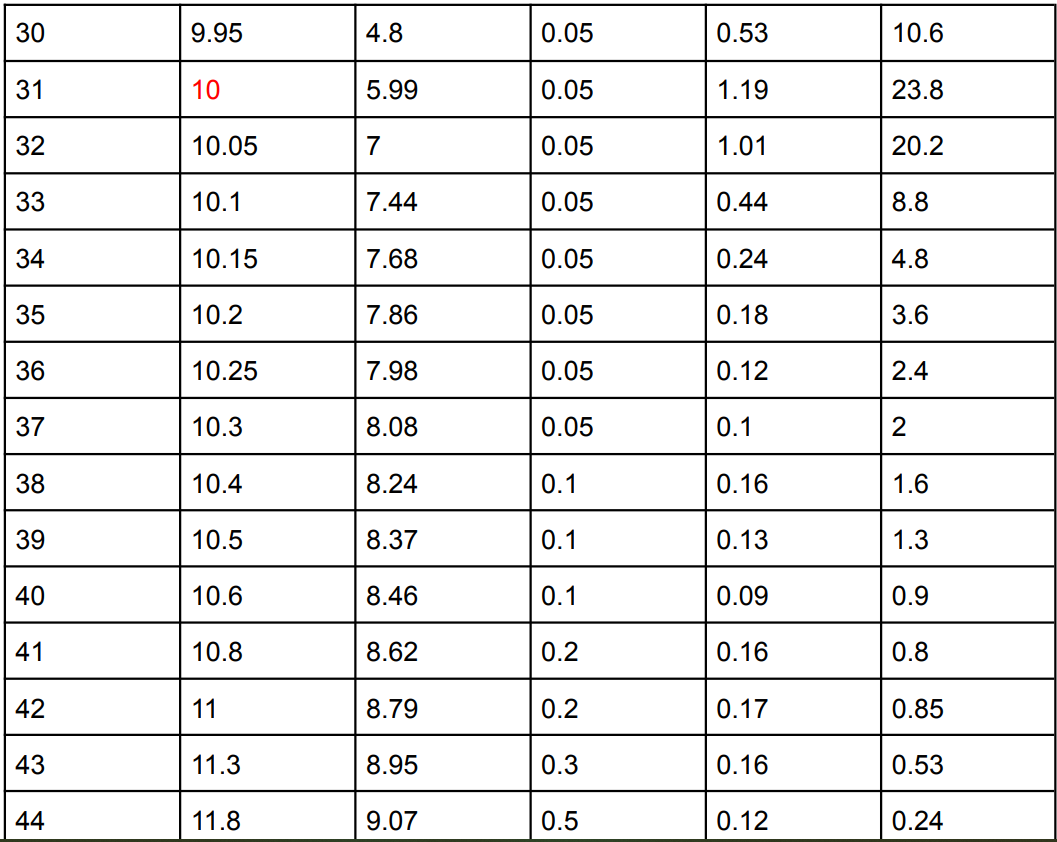
\includegraphics[scale=0.7]{table4}
	\end{figure}
	\begin{figure}[H]
		\centering
		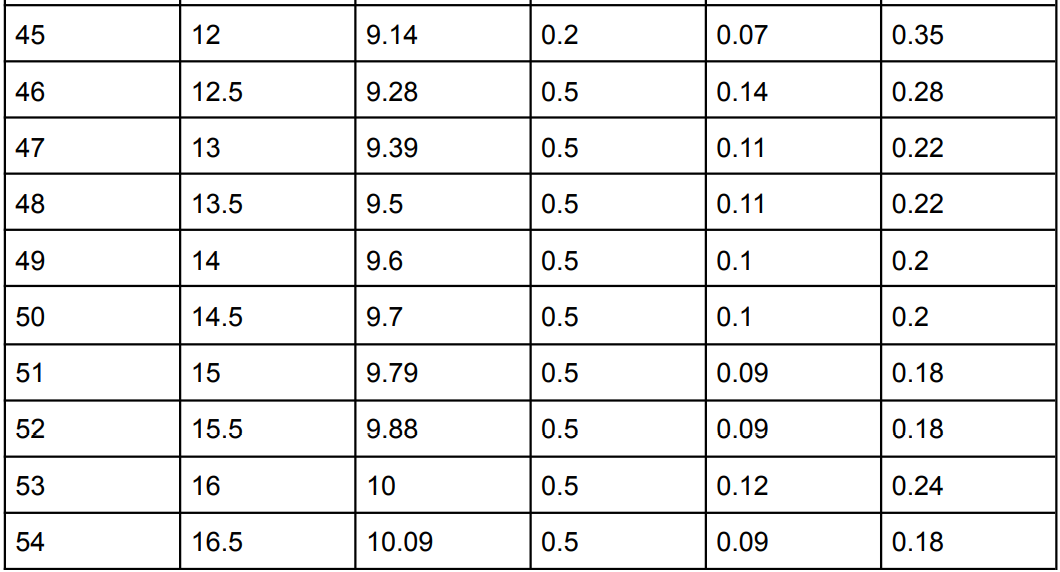
\includegraphics[scale=0.7]{table5}
	\end{figure}
	\begin{figure}[H]
		\centering
		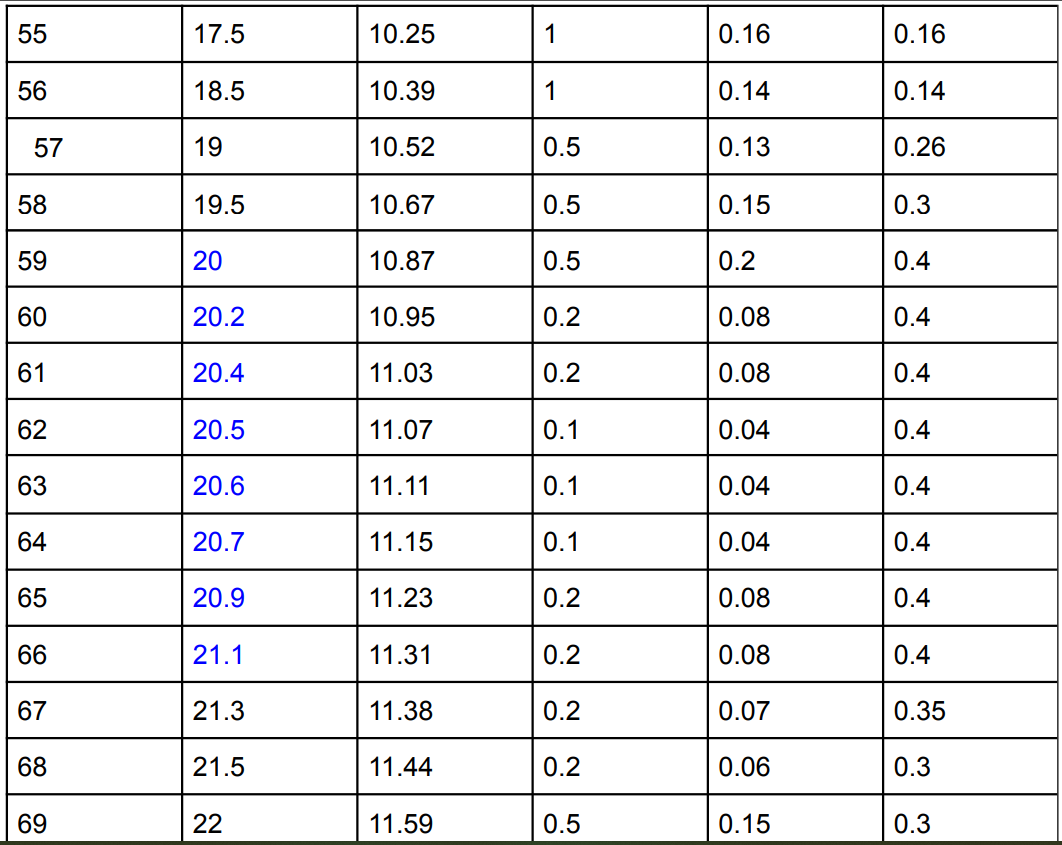
\includegraphics[scale=0.7]{table6}
	\end{figure}
	\begin{figure}[H]
		\centering
		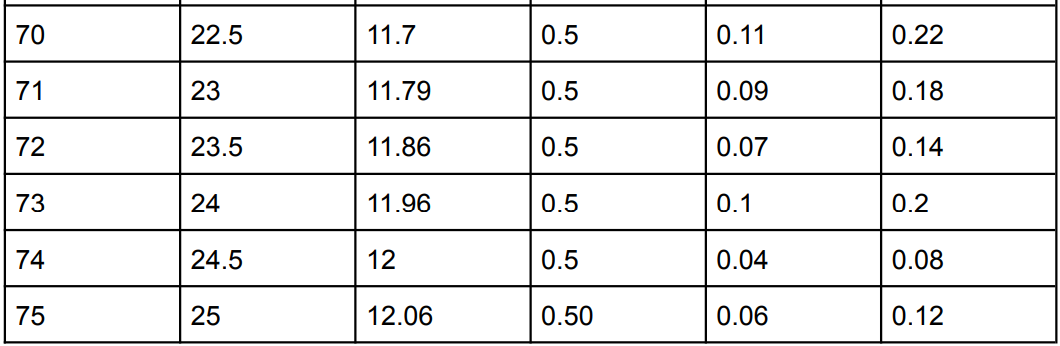
\includegraphics[scale=0.7]{table7}
	\end{figure}

	\section{Plots}
	
	\begin{figure}[H]
		\centering
		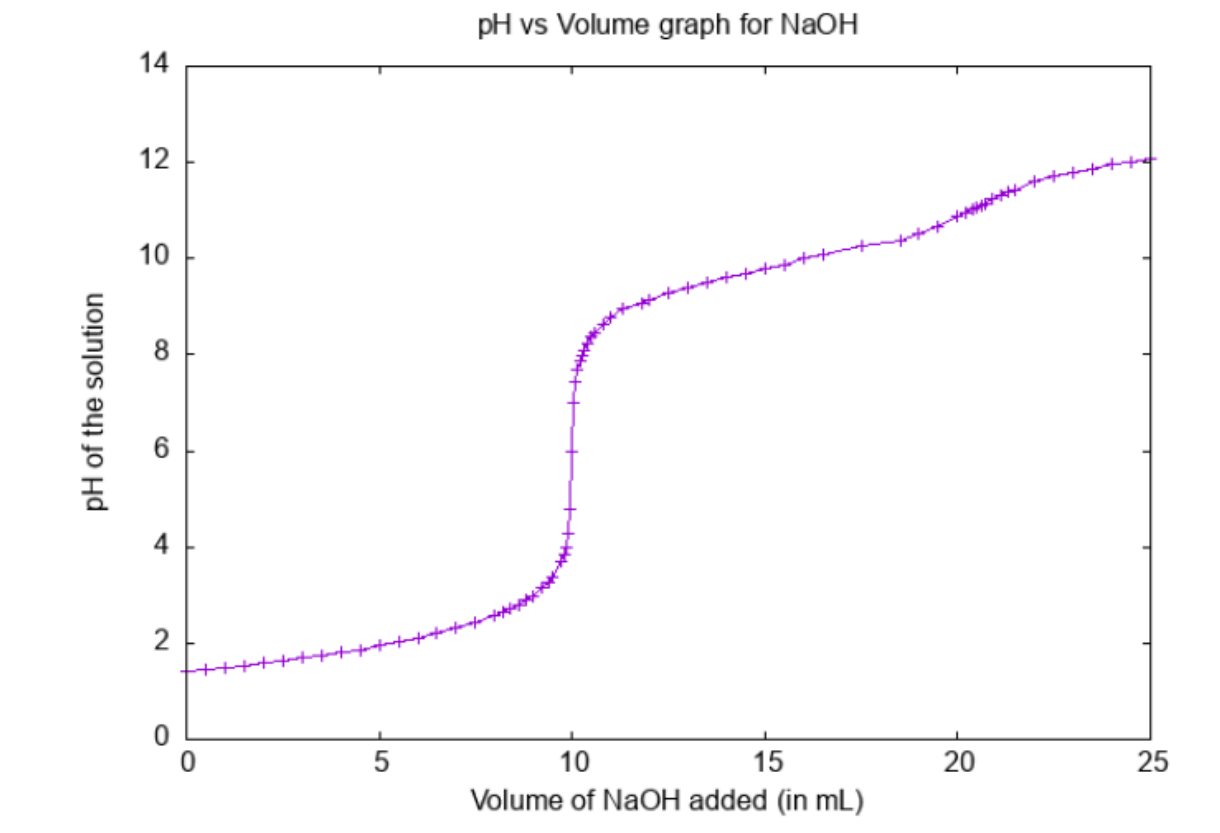
\includegraphics[scale=0.7]{plot1}
		\caption{pH vs Volume graph for NaOH }
	\end{figure}

	\begin{figure}[H]
		\centering
		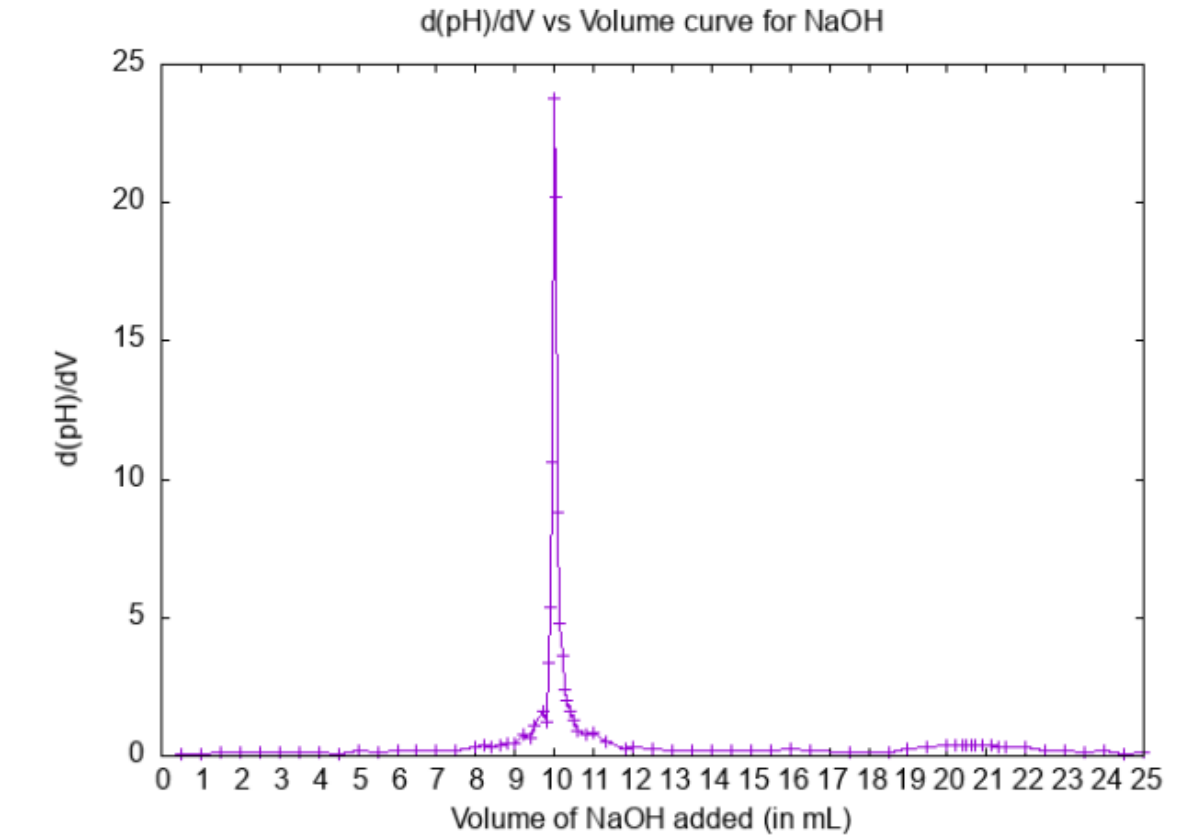
\includegraphics[scale=0.7]{plot2}
		\caption{$\frac{\Delta pH}{\Delta V}$ vs Volume curve}
	\end{figure}
	
	\section{Results and Data Interpretation}
	
	From the second plot above, it is clear that there are two equivalence points (since
	there are two peaks : first between 9 mL and 11 mL and second between 20 mL and 21
	mL).
	
	\emph{\underline{First Equivalence Point :}}
	
	The first equivalence point corresponds to volume = 10 mL {\color{red}(shown in RED in
	Table 3)}
	So, half equivalence point = 5 mL
	From Table 3, $pK_{a}$ value corresponding to first half equivalence point, $pK_{a_{1}}$ = 1.95
	
	\emph{\underline{Second Equivalence Point :}}
	
	For the second equivalence point there is no single point peak. Instead 8 different
	volume readings correspond to the local maximum value of $pK_{a}$ {(\color{blue}shown in BLUE
	in Table 3)}
	
	So, we take the average of the 8 volume readings to find the ‘Second Equivalence
	Point’ as below:
	
	Volume at second equivalence point $= \dfrac{20+20.2+20.4+20.5+20.6+20.7+20.9+21.1}{8} = 20.55 mL$
	
	So, the half equivalence point $= \dfrac{First\ Eq.\ Point\ +\ Second\ Eq.\ Point}{2} = \dfrac{10+20.55}{2} = 15.275 mL$
	
	From the Table, $pK_{a}$ value nearest to second half equivalence point, = 9.88
	
	Now, we know that,
	
	Equivalence Point (pI) $= \dfrac{pK_{a_{1}} + pK_{a_{2}}}{2} = \dfrac{1.95 + 9.88}{2} = 5.915$
	
	Thus, pI $= 5.915$
	
	\section{Conclusion}
	
	The Isoelectric Point of the given Amino Acid (Glycine) is \underline{5.915}.\footnote{All the graphs were plotted using \emph{gnuplot}}.
\end{document}